\documentclass[12pt]{article}
\usepackage[utf8]{inputenc}
\usepackage{amsmath}
\usepackage[T1]{fontenc}

\title{ECE 3413 Lab 10\\*Closed Loop Gain Determination using Root Locus}
\author{Leomar Dur\'an}
\date{${23}^{\text{th}}$ April 2023}

\usepackage[natbib,style=apa6]{biblatex}
\addbibresource{main.bib}
\defbibheading{bibliography}[\refname]{%
  \section*{\centering #1}%
}%

\usepackage{hyperref}

\usepackage{cancel}
\usepackage[per-mode=symbol]{siunitx}
\newcommand*\siexpr[2][]{\SI[parse-numbers=false,#1]{#2}}%
\DeclareSIUnit\bel{B}
\DeclareSIUnit\byte{Byte}

\usepackage{xfrac}
\usepackage{amssymb}
\newcommand*\transpose{\mathsf{T}}

\usepackage{mathtools}%
\DeclarePairedDelimiter\brao()%
\DeclarePairedDelimiter\brac[]%
\DeclarePairedDelimiter\braco[)%
\DeclarePairedDelimiter\braoo][%
\DeclarePairedDelimiter\Brac\{\}%
\DeclarePairedDelimiter\abs||
\DeclarePairedDelimiter\norm\lVert\rVert%
\DeclarePairedDelimiter\piecefn\{.
\DeclarePairedDelimiter\evalat.|

\usepackage{lib/nonfloatenvirons}
\usepackage{booktabs}
\newcommand\ra[1]{\renewcommand*\arraystretch{#1}}
\ra{1.25}

\usepackage{minted}
\newcommand\matlab{matlab}

\usepackage{adjustbox}
\newcommand{\setprime}[2][1]{%
    {#2}^{%
        \raisebox{1pt}{%
            \scalebox{0.5}{%
                \itshape\sffamily\uppercase%
                \expandafter{%
                    \romannumeral#1%
                }%
            }%
        }
    }%
}%
\newcommand*\mcadj[7]%
% {#columns}{col spec}{rotation}{adjust spec}
% {before rotated text}{rotated text}{after rotated text}
{%
    \multicolumn{#1}{#2}{%
        \rlap{%
            #5\adjustbox{rotate=#3,#4}{#6}~#7%
        }%
    }%
}

\usepackage{pdfpages}
\usepackage{standalone}
\usepackage{matlab}

\usepackage[skip=\baselineskip,indent=0pt]{parskip}
\setlength\parindent{0pt}

\usepackage[shortlabels]{enumitem}

\def\hr{{\par\noindent\rule{\textwidth}{0.4pt}}}

\begin{document}

\maketitle
\newpage

\section{Introduction}\label{sec:intro}

\subsection{The setup}\label{ssc:the setup}

For this lab,
we will need to install the System Identification Toolbox add-on.

Before starting the installation,
be warned that the installation will require escalation to Administrator privileges.
One will also need to agree to ``The MathWorks, Inc. Software License Agreement''
as the System Identification Toolbox add-on as created by MathWorks%
{} (as of this writing).
After the installation, \textsc{Matlab} will restart,
so save all previous work first.

Additionally,
this add-on has no additional dependencies.
The download is $\SI{61}{\mega\byte}$ and the installation is $\SI{160}{\mega\byte}$.

\begin{enumerate}
    \item
        Once ready,
        open the Home tab,
        and find the Add-Ons menu in the \textsc{environment} section
        as shown in Fig.~\ref{fig:finding addons},
        and click the Get Add-Ons button highlighted.

        \begin{figure}
            \centering
            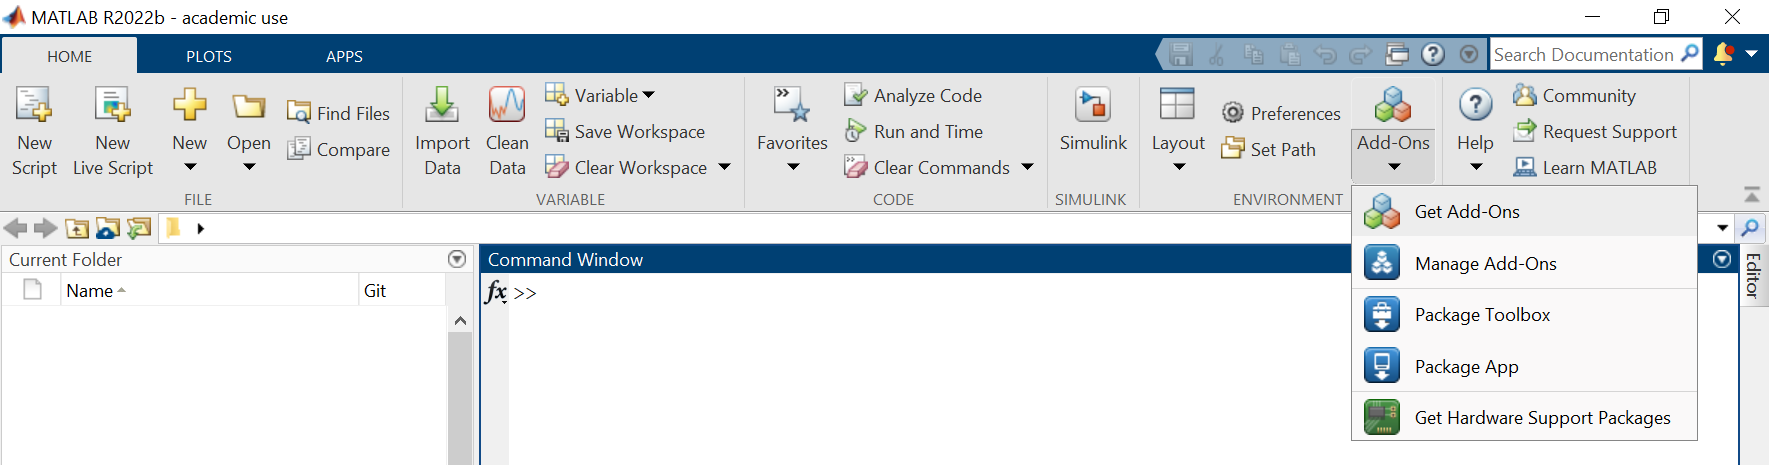
\includegraphics[width=\linewidth]{img/intro_010_finding_addons.png}
            \caption{Finding the Add-Ons menu.}
            \label{fig:finding addons}
        \end{figure}

    \item
        In the search bar of the ``Add-On Explorer'' dialog opened,
        search for ``Simulation Control Design''.
        It is the first hit in the results listed in Fig.~\ref{fig:searching System Identification Toolbox}.

        \begin{figure}
            \centering
            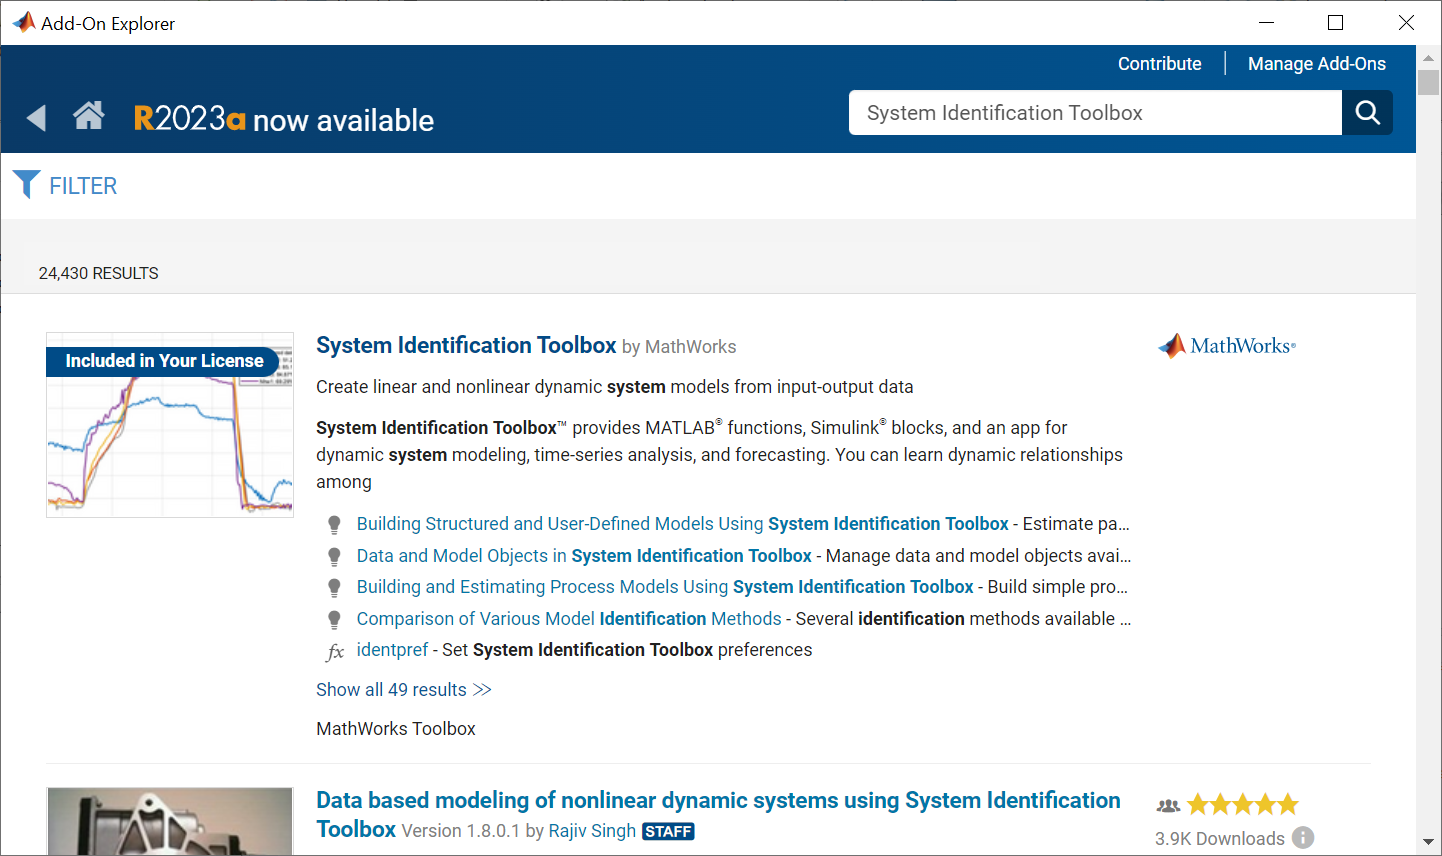
\includegraphics[width=\linewidth]{img/intro_020_searching_system_id_toolbox.png}
            \caption{The ``Add-On Explorer'' dialog with ``Simulation Control Design'' hovered in navy blue text.}
            \label{fig:searching System Identification Toolbox}
        \end{figure}

        The Simulation Control Design add-on should be labeled
        with the navy blue ``Included In Your License'' label.
        However,
        if it was already installed,
        then you will see the green ``Installed'' label%
        {} seen in Fig.~\ref{fig:searching ìnstalled System Identification Toolbox},
        in which case,
        no further action is needed
        and you may proceed to Subsection~\ref{ssc:background} \nameref{ssc:background}.

        \begin{figure}
            \centering
            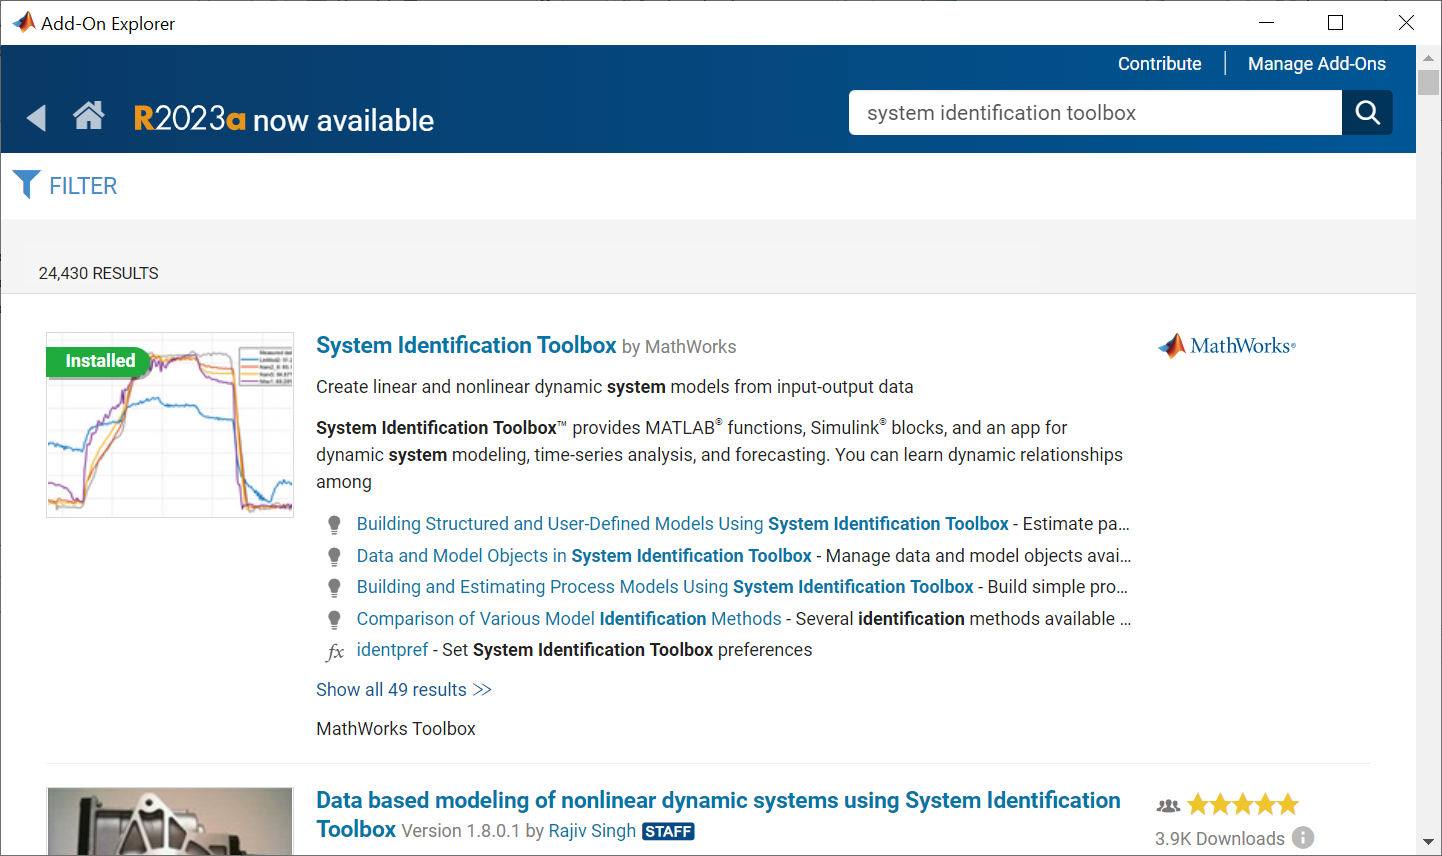
\includegraphics[width=\linewidth]{img/intro_050_searching_installed_system_id_toolbox}
            \caption{The Simulation Control Design add-on already installed in the ``Add-On Explorer'' dialog.}
            \label{fig:searching ìnstalled System Identification Toolbox}
        \end{figure}

        However, if the label is different from either of these,
        please contact your administrator about licensing%
        {} before proceeding.

        Proceeding from Fig.~\ref{fig:searching System Identification Toolbox},
        click on the Simulation Control Design add-on to select it.
    \item
        To install,
        click on the Install button,
        which will highlight in light blue when hovered over like in Fig.~\ref{fig:selected System Identification Toolbox}.

        \begin{figure}
            \centering
            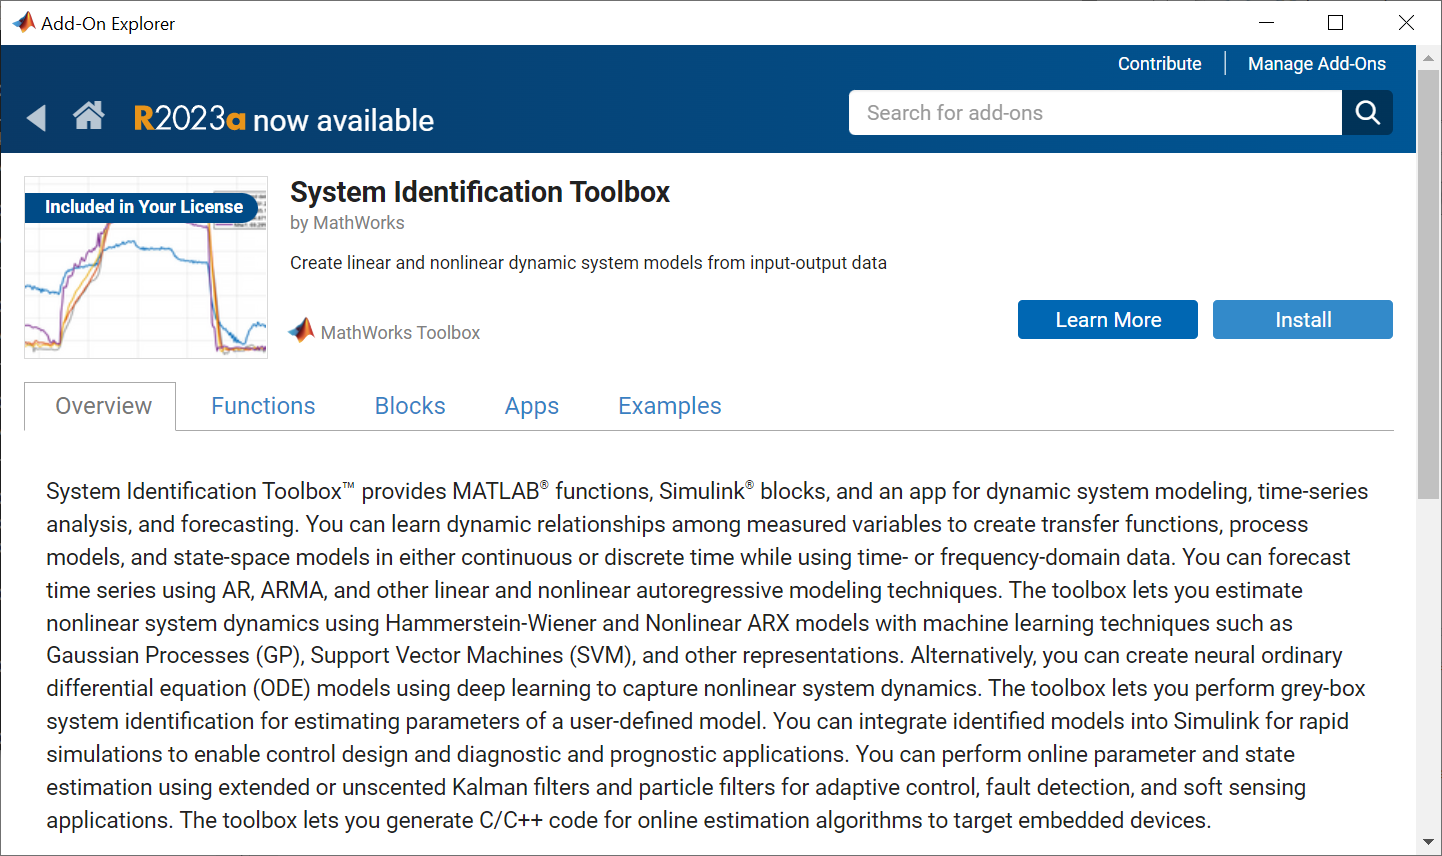
\includegraphics[width=\linewidth]{img/intro_030_selected_system_id_toolbox.png}
            \caption{The Simulation Control Design add-on selected and ready for installation.}
            \label{fig:selected System Identification Toolbox}
        \end{figure}

        Follow the onscreen instructions,
        which will include escalation to Administrator privileges
        and agreeing to the ``The MathWorks, Inc. Software License Agreement''.

    \item
        \textsc{Matlab} will complete the installation process and restart,
        after which you will be greeted by the dialog in \ref{fig:System Identification Toolbox installation finished}.

        \begin{figure}
            \centering
            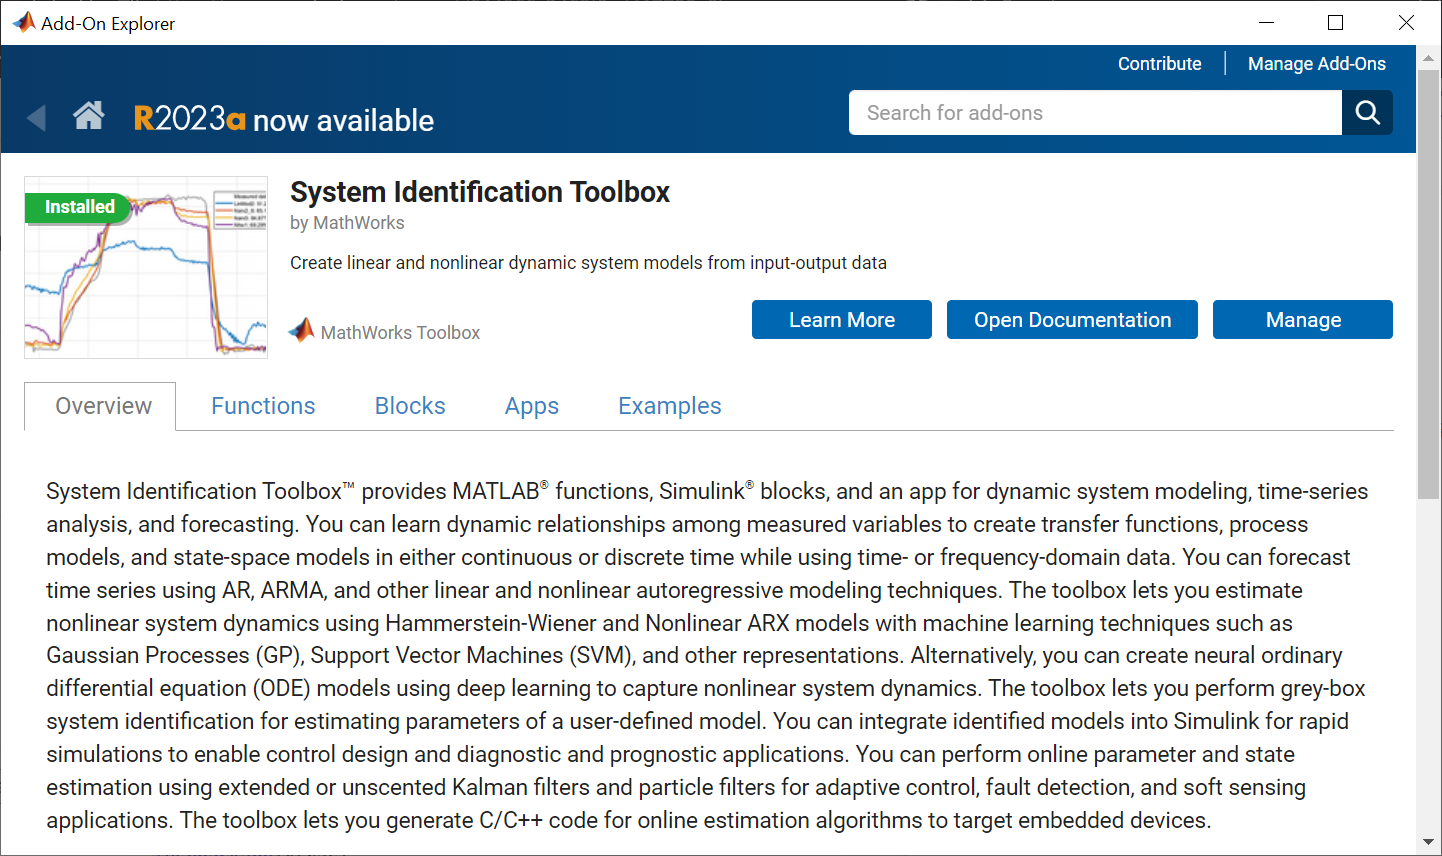
\includegraphics[width=\linewidth]{img/intro_040_installed_system_id_toolbox.png}
            \caption{Dialog showing complete installation of the Simulation Control Design add-on.}
            \label{fig:System Identification Toolbox installation finished}
        \end{figure}
\end{enumerate}
\newpage

\subsection{Background information}\label{ssc:background}

This experiment builds on the previous lab (DC Motor Model for Open-loop Control in \textsc{Matlab} Simulink) by providing a PID (proportional-integral-derivative) feedback controller to stabilize the angular velocity.

As we saw earlier, the angular velocity will rise increasingly until it reaches the desired velocity and plateaus. Fig.~\ref{fig:plot of angular velocity} shows this increment of angular velocity.

\begin{figure}
    \centering
    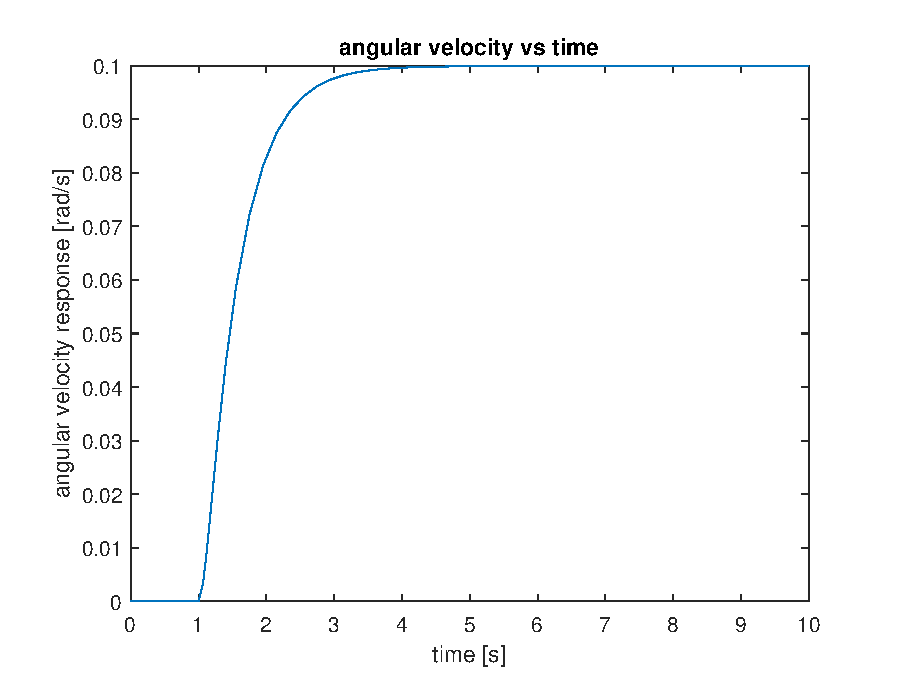
\includegraphics[width=\linewidth]{img/task02_plot_angular_velocity.eps}
    \caption{Plot of the angular velocity response.}
    \label{fig:plot of angular velocity}
\end{figure}

From this, we can expect the angular position to increase equally throughout the runtime as we see in Fig.~\ref{fig:angular position of motor}.

\begin{figure}
    \centering
    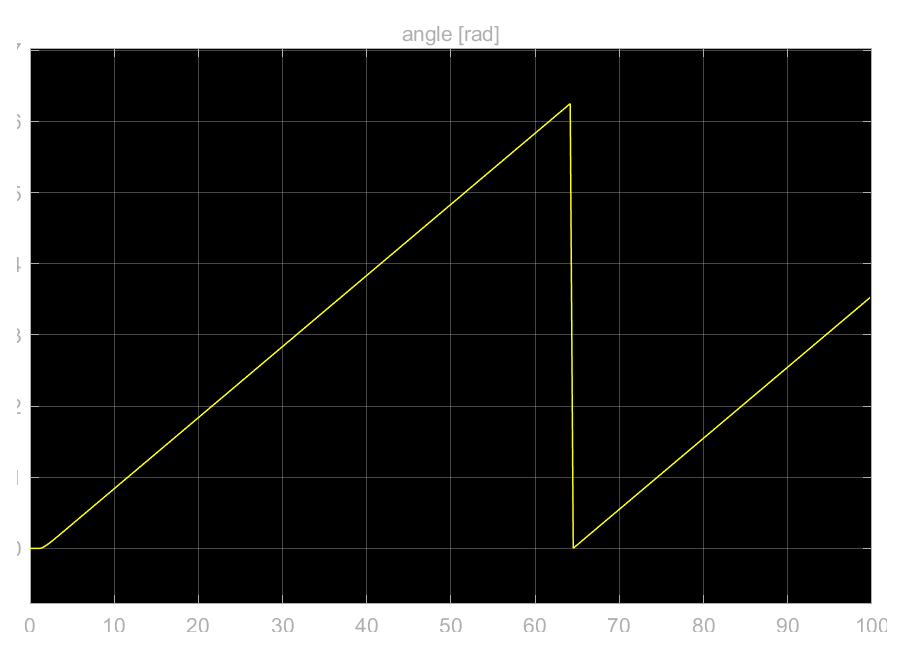
\includegraphics[width=\linewidth]{img/task05_angular_position.eps}
    \caption{The angular position of the motor.}
    \label{fig:angular position of motor}
\end{figure}

However, it may be desired to change the output of the motor. In which case, we can use a PID controller to stabilize this change according to whichever parameter we desire.

These parameters may include wanting the system to be overdamped (for more stead changes) or underdamped (for quicker changes).

\section{Proceedure}\label{sec:Proceedure}

\subsection{Task 00 -- Adding the PID controller}\label{ssc:dc motor model}

We start with the DC motor model from the previous lab as shown on pages~\pageref{pdf:dc motor model} and \pageref{pdf:integrators}.

However, to the original system from lab~08, we are adding a PID controller and a negative unit feedback loop as seen on page~\ref{pdf:PID controller system}.

\begin{figure}
    \centering
    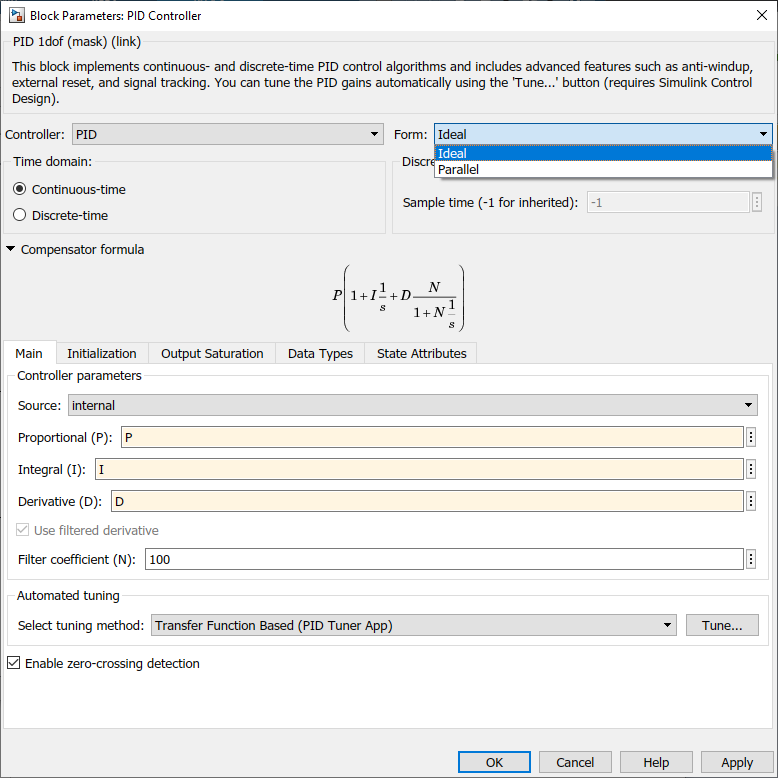
\includegraphics[width=\linewidth]{img/task00_010_setting_up_PID_controller.png}
    \caption{Setting up the PID controller.}
    \label{fig:pid controller block parameters}
\end{figure}

Additionally, to set up the PID controller, we must edit the block parameters as seen in Fig.~\ref{fig:pid controller block parameters}. We have made the following changes:
\begin{enumerate}
    \item Change the Form from ``Parallel'' to ``Ideal''.
    \item Set Proportional (P) to \mintinline\matlab{P}.
    \item Set Integral (I) to \mintinline\matlab{I}.
    \item Set Derivative (D) to \mintinline\matlab{D}.
\end{enumerate}

We can see the general form of the compensator formula here, that is
\begin{equation}\label{eq:ideal compensator}
    P\brao*{1 + I\frac1s + D\frac{N}{\displaystyle1 + N\frac1s}}\rlap.
\end{equation}

\begin{figure}
    \centering
    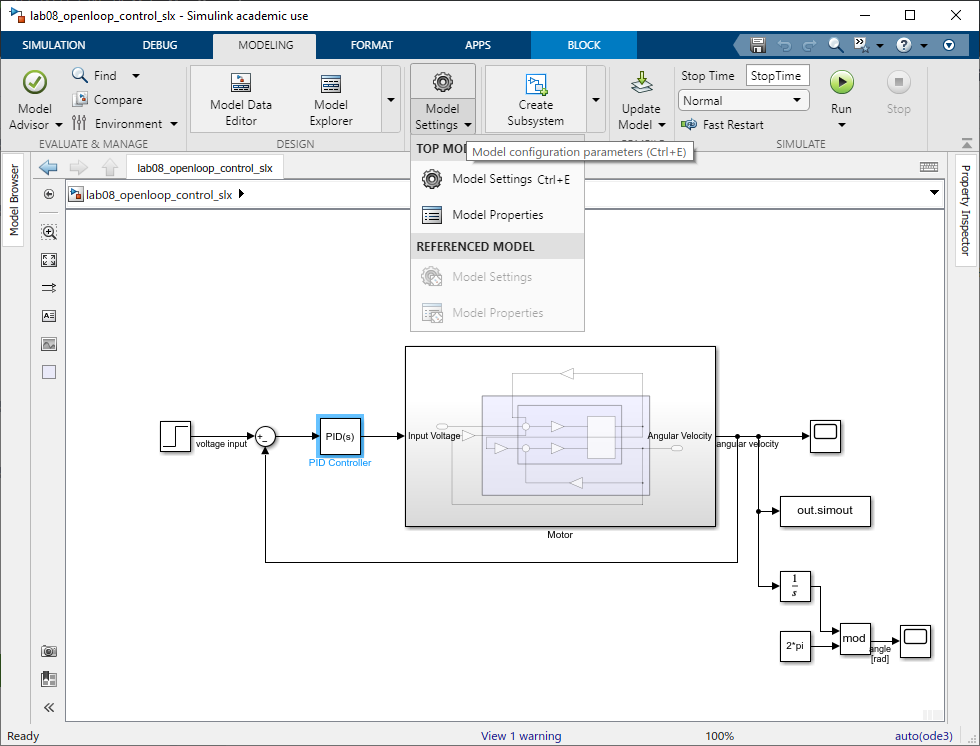
\includegraphics[width=\linewidth]{img/task00_020_finding_model_settings.png}
    \caption{Locating the model settings.}
    \label{fig:task00_020_finding_model_settings}
\end{figure}

\includepdf[pages=2,landscape=true,pagecommand=\label{pdf:dc motor model}]{drawings/lab09_pid_feedback_control_slx.pdf}
\includepdf[pages=3,landscape=true,pagecommand=\label{pdf:integrators}]{drawings/lab09_pid_feedback_control_slx.pdf}
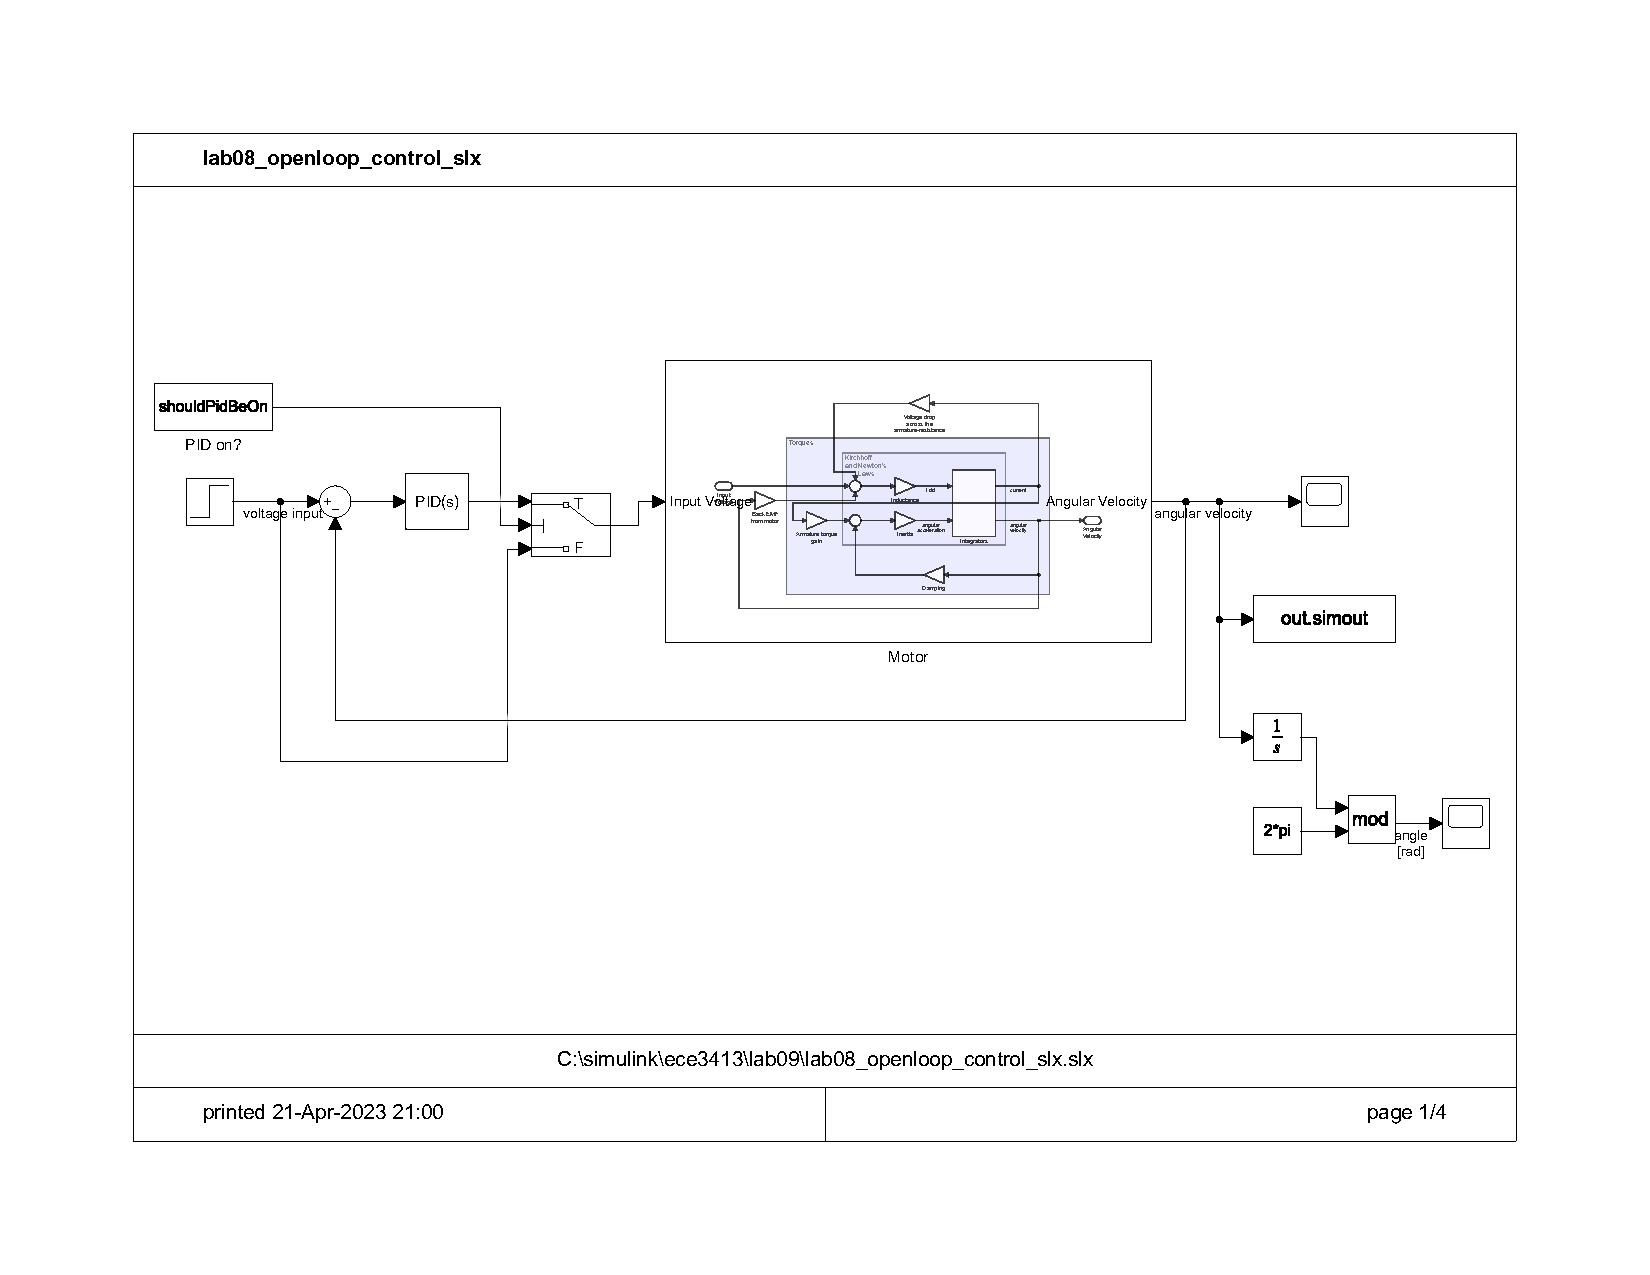
\includepdf[pages=1,landscape=true,pagecommand=\label{pdf:PID controller system}]{drawings/lab09_pid_feedback_control_slx.pdf}

We will also need to change the Model Settings. These can be found by clicking on the ``MODELING'' tab at the top of the Simulink window. Then selecting the Model Settings with the gear icon near the middle as see in \ref{fig:task00_020_finding_model_settings}.

The settings that we changed are as follows:
\begin{enumerate}
    \item Add a Start time of \mintinline\matlab{StartTime}.
    \item Set the Solver selection to ``Fixed-step''.
    \item Set the Fixed-step size, which is the sampling frequency to \mintinline\matlab{Fs}.
\end{enumerate}

Now these settings are all parameterized by the script in \nameref{app} subsection~\ref{sap:initial params}.

\subsection{Task 01 -- Varying the proportional terms}

We plotted the result of modeling the PID feedback system as a purely proportional system with the proportional terms given in \eqref{eq:proportional}.

\begin{equation}\label{eq:proportional}
    P \in \Brac*{10^n\middle| n \in 0..3^{\vphantom1}}\rlap.
\end{equation}

We automated this process by using the script in \nameref{app} subsection~\ref{sap:vary p}.

\subsection{Task 02 -- Varying the proportional, integral terms}

We plotted the result of modeling the PID feedback system as a PI system, varying both the proportional and integral terms as given in \eqref{eq:proportional, integral}.

\begin{equation}\label{eq:proportional, integral}
    \brao{I, P} \in \brac*{
        \begin{matrix}
            0.1 & 100 \\*
            0.5 & 100 \\*
            1 & 100 \\*
            1 & 10 \\*
        \end{matrix}
    }\rlap.
\end{equation}

We automated this process by using the script in \nameref{app} subsection~\ref{sap:vary pi}.

\subsection{Task 03 -- Varying the proportional terms}

We plotted the result of modeling the PID feedback system with constant proportional term $P = 10$, constant integral term $I = 1$, and varying derivative terms given in \eqref{eq:derivative}.

\begin{equation}\label{eq:derivative}
    D \in \Brac*{10^n\middle| n \in 0..2^{\vphantom1}}\rlap.
\end{equation}

We automated this process by using the script in \nameref{app} subsection~\ref{sap:vary d}.

\subsection{Task 07 -- Tuning with the Simulink PID Tuner application}\label{ssc:Simulink PID Tuner application}

\begin{figure}
    \centering
    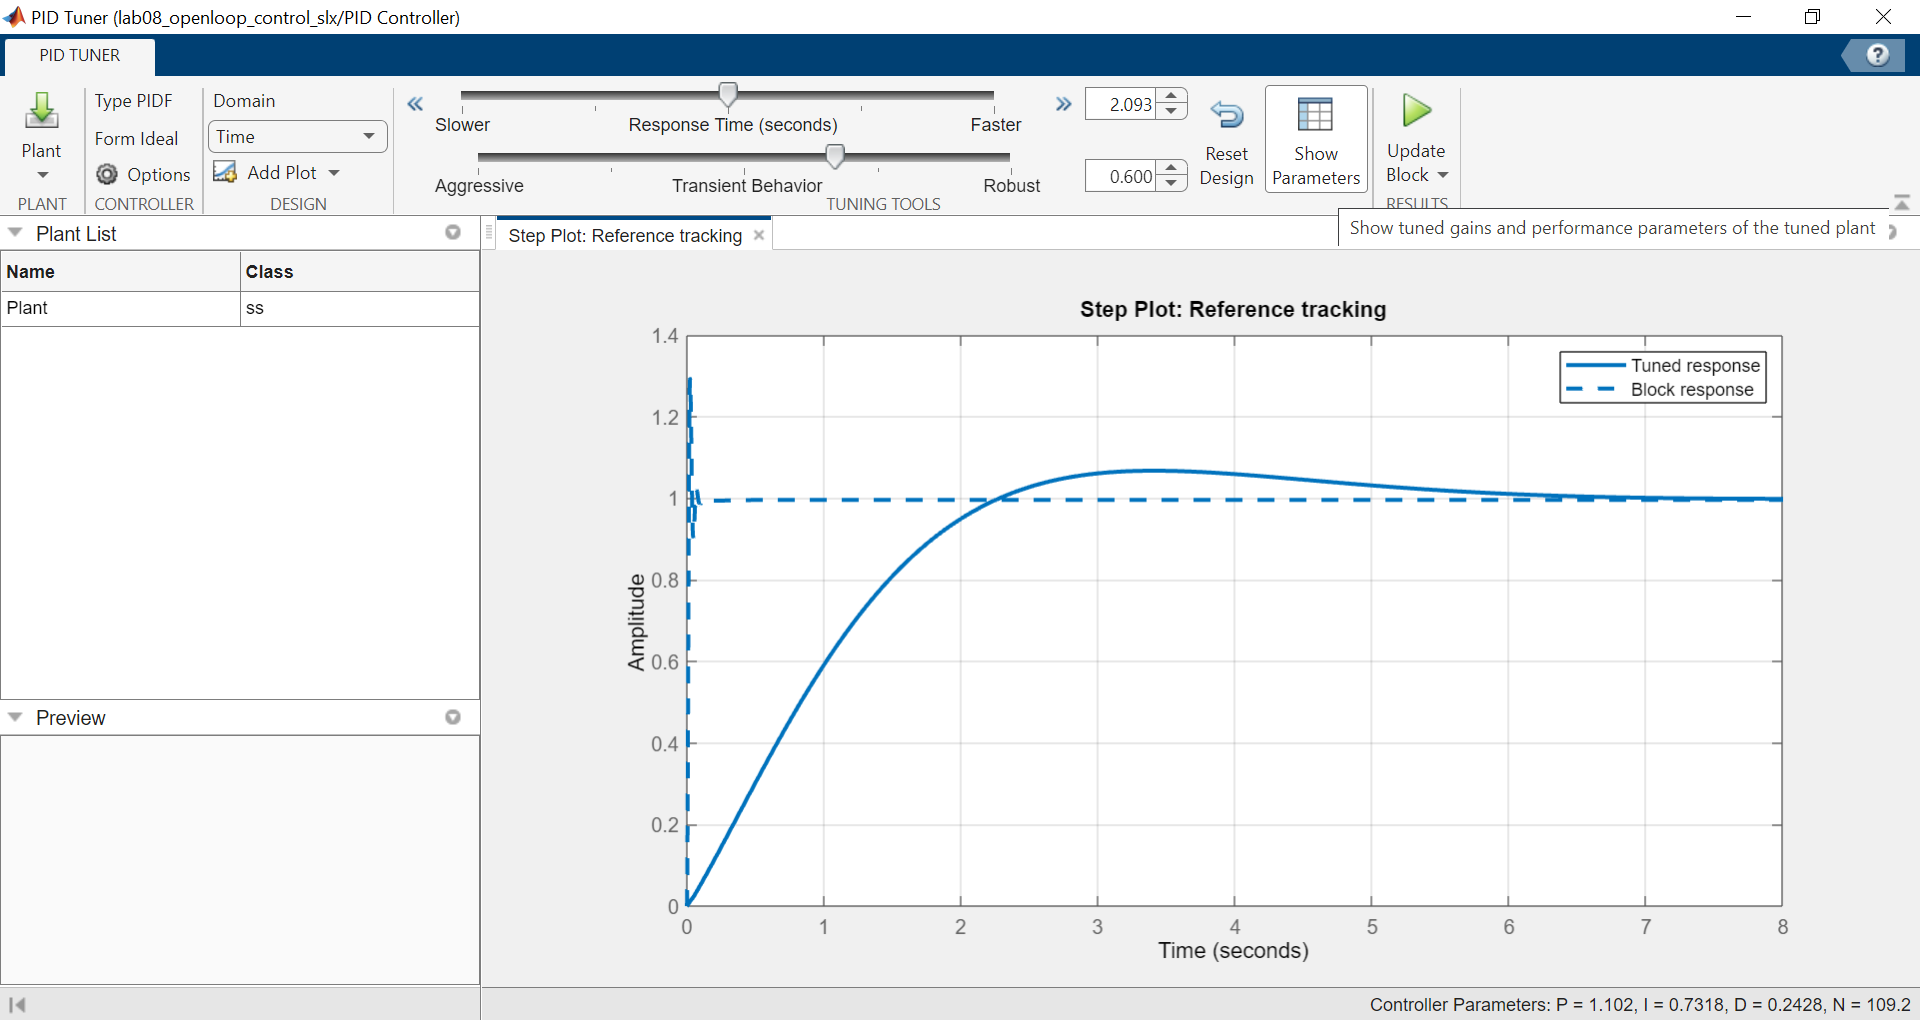
\includegraphics[width=\linewidth]{img/task07_010_default_tuning.png}
    \caption{Default PID tuning with the ``Show Parameters'' button highlighted.}
    \label{fig:task07_010_default_tuning}
\end{figure}

If you have not done so yet,
install the System Identification Toolbox add-on as outlined in the \ref{sec:intro} subsection~\ref{ssc:the setup},
or the next step will not work.

Open the PID controller in the Simulink model
and you will see \ref{fig:pid controller block parameters}.
Here click the ``Tune\dots'' button in the ``Automated tuning'' field set. This will open the PID Tuner dialog in \ref{fig:task07_010_default_tuning}.
The highlighted button ``Show Parameters'' opens a window to the parameters that configure the tuned PID
as seen in \nameref{app} subsection~\ref{sap:tuned PID parameters reference table}.

In the \nameref{sec:Discussion}, we discuss the parameters for a cruise control, coming to the conclusion that we will need a control with $P < 10$, $I < 1$, and $D = 0$.

Let us choose a robust control and find the fastest response time that will meet these requirements.
This produces the transfer function whose step response is seen in Fig.~\ref{fig:task07_020_cruise_control}.

\begin{figure}
    \centering
    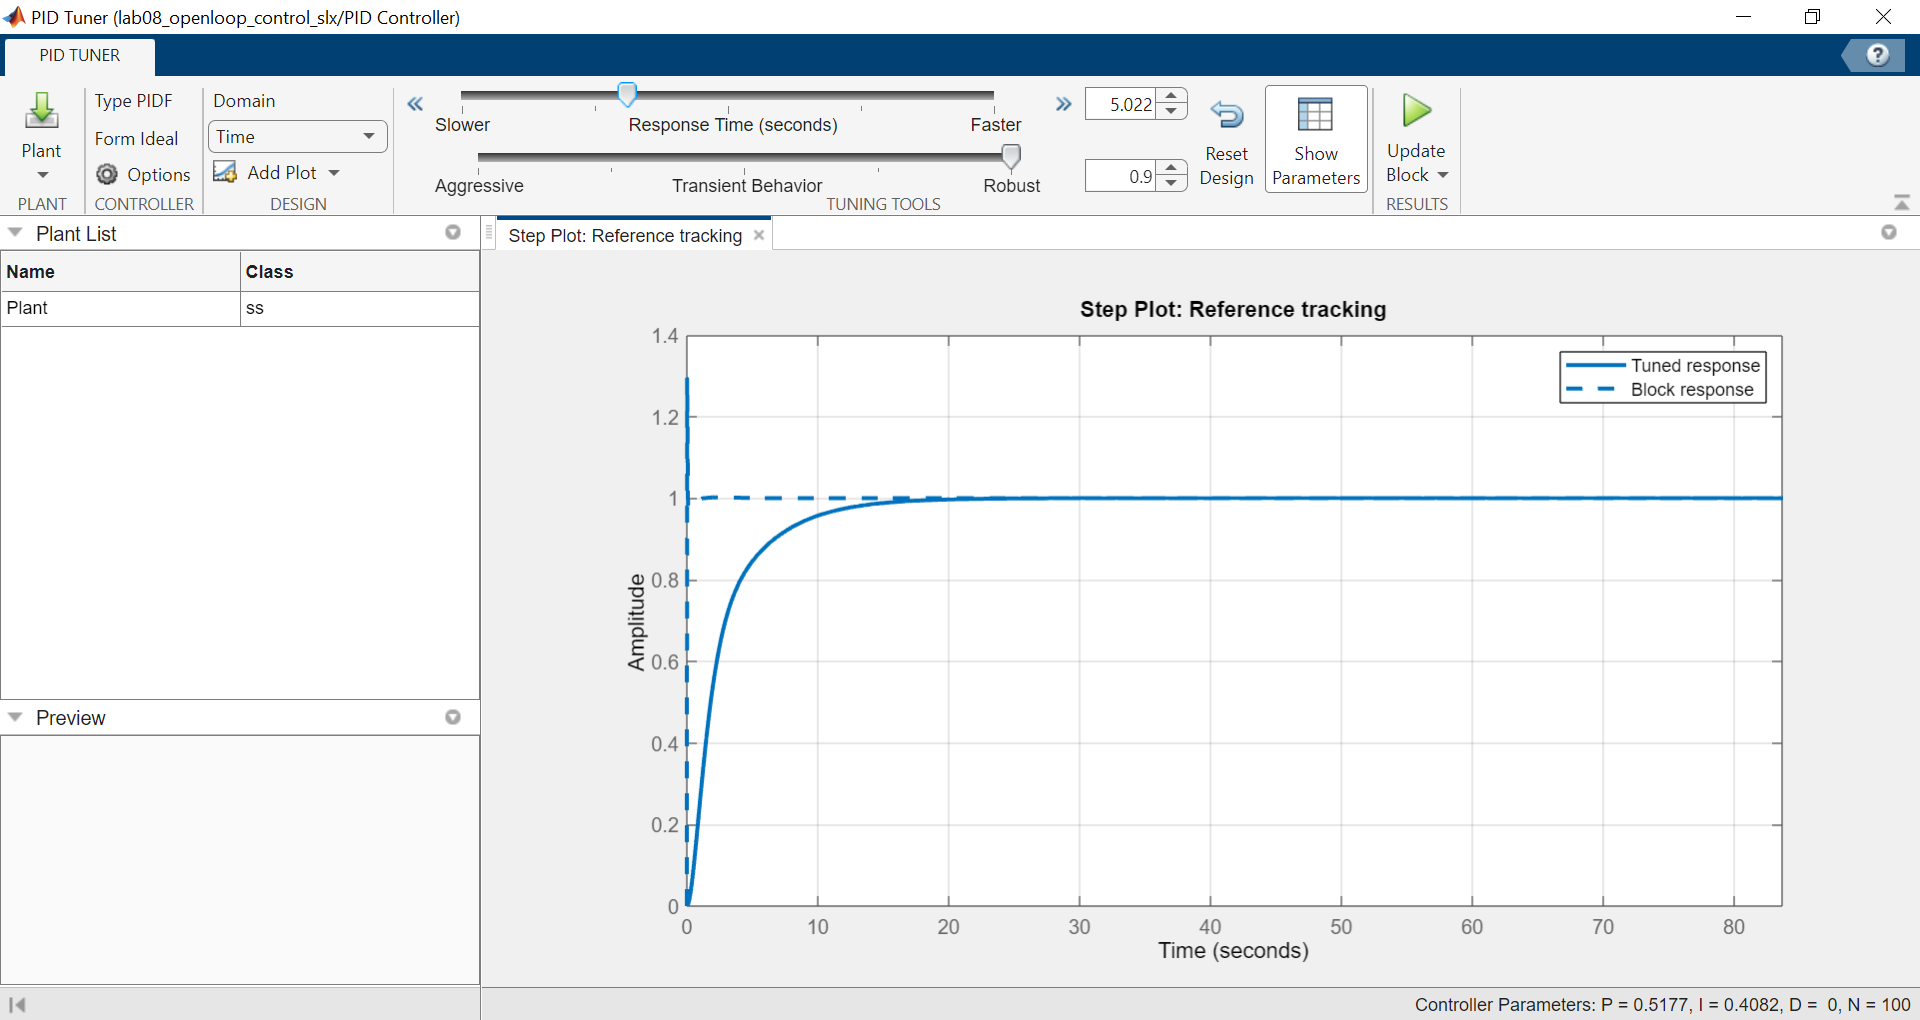
\includegraphics[width=\linewidth]{img/task07_020_cruise_control.png}
    \caption{The PID tuning chosen for a cruise control.}
    \label{fig:task07_020_cruise_control}
\end{figure}

We can see that compared to the block response showing our initial parameters from the script in \nameref{app} subsection~\ref{sap:initial params},
that there is no overshoot,
and in fact the new step response seems near critically damped,
however, it has a settling time much higher in magnitude (about $220\times$).

Further increasing the speed by reducing the step time by $\SI{0.226}\second$ for comparison, which is seen in \nameref{app} subsection~\ref{sap:faster than cruise, step response}.
This PID controller is too fast and produces an overshoot.

We produce the parameters shown in Table \ref{tab:tuned vs block reponse params}.

\begin{table}[]
    \centering
    \caption{Parameters of the tuned response vs block response.}
    \[
        \begin{array}{@{}*5l@{}}
            \toprule
                &
                    & \text{Tuned}
                    & \text{Faster}
                    & \text{Block} \\*
            \midrule
                \text{Response time} & \brac{\si\second}
                    & 5.022 & 4.796 & - \\*
                \text{Transient behavior} &
                    & 0.9 & 0.9 & - \\*
            \midrule
                P && 0.51773 & 0.31862 & 100 \\*
                I && 0.40823 & 0.89342 & 1 \\*
                D && 0 & 0 & 1 \\*
                N && 100 & 100 & 100 \\*
            \midrule
                \text{Rise time} & \brac{\si\second}
                    & 6.16 & 3.52 & 0.0099
                \\*
                \text{Settling time} & \brac{\si\second}
                    & 13 & 9.36 & 0.0598
                \\*
                \text{Overshoot} &
                    & \SI{0}\percent & \SI{3}\percent & \SI{29.2}\percent
                \\*
                \text{Peak} &
                    & 1 & 1.03 & 1.29
                \\*
                \text{Gain margin} & \brac{\si{\deci\bel}}
                    & \infty & \infty & \infty
                \\*
                \text{Gain margin frequency} & \brac{\si{\radian\per\second}}
                    & \infty & \infty & \infty
                \\*
                \text{Phase margin} & 
                    & \SI{90}\degree & \SI{69}\degree & \SI{39.2}\degree
                \\*
                \text{Phase margin frequency} & \brac{\si{\radian\per\second}}
                    & 0.398 & 0.417 & 126
                \\*
                \text{Closed-loop stability} &
                    & \text{Stable}
                    & \text{Stable}
                    & \text{Stable}
                \\*
            \bottomrule
        \end{array}
    \]
    \label{tab:tuned vs block reponse params}
\end{table}

As expected the Tuned response has
$P := 0.51773 < 10$,
$I := 0.40823 < 1$,
and $D := 0$.
We have produced an overshoot of $\SI0\percent$
with as low a rise time, so that lower a rise time will produce overshoot.
This is ideal for cruise control.

\section{Results}

\subsection{Task 01 -- Varying the proportional terms}

\begin{figure}
    \centering
    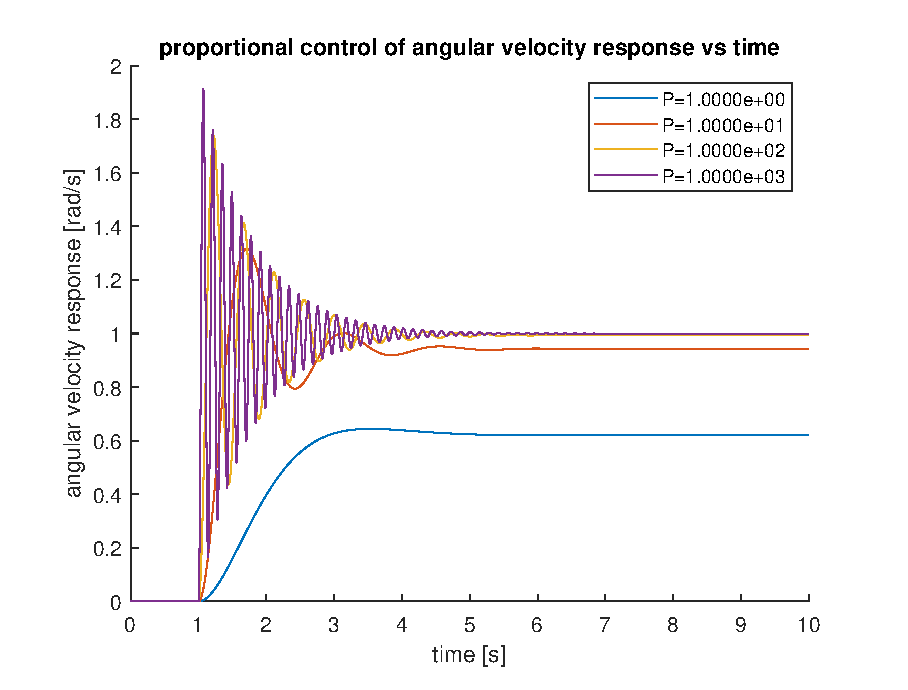
\includegraphics[width=\linewidth]{img/task01_varying_p.eps}
    \caption{Effect of the proportional term the angular velocity response in a proportional controller.}
    \label{fig:p on angular velocity}
\end{figure}

The effect of the proportional term on the response is twofold.
\begin{enumerate}
    \item There is a diminishing effect on the amplitude of the signal, but the percent overshoot continues to increase.
    \item The system becomes less damped to the point of increasing in oscillations as the $P$ term increases.
\end{enumerate}

\subsection{Task 02 -- Varying the proportional, integral terms}

\begin{figure}
    \centering
    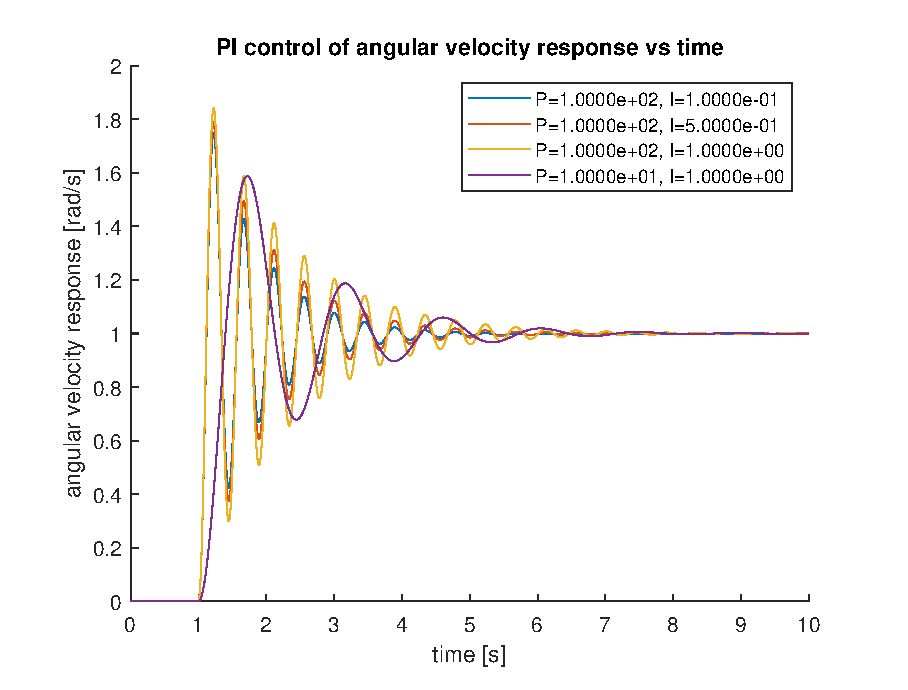
\includegraphics[width=\linewidth]{img/task02_varying_pi.eps}
    \caption{Effect of the proportional and integral terms the angular velocity response in a PI controller.}
    \label{fig:pi on angular velocity}
\end{figure}

The integral term has no effect on damping, it only changes the percent overshoot, but the number of oscillations remains the same. The change that we see in the last curve is because of the decrease in the proportional term.

\subsection{Task 03 -- Varying the proportional terms}

\begin{figure}
    \centering
    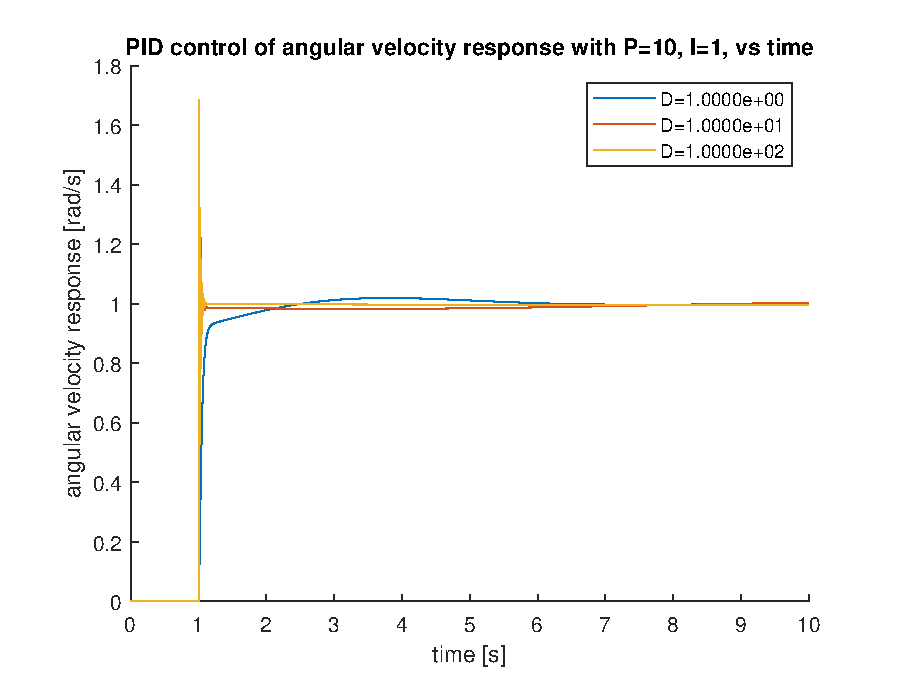
\includegraphics[width=\linewidth]{img/task03_varying_d.eps}
    \caption{Effect of the derivative term the angular velocity response in a PID controller.}
    \label{fig:d on angular velocity}
\end{figure}

All of these curves seem to have very quick settling times. The difference is that the derivative term creates a very dramatic effect on the percent overshoot. However, unlike the derivative term, it settles much more quickly.

\section{Discussion}\label{sec:Discussion}

\subsection{Parallel PID controllers}

Besides the ideal PID controller that we have been using,
there exist parallel PID controllers,
and the difference between them
is that a parallel uses the compensator formula

\begin{equation}
    P + I\frac1s + D\frac{N}{\displaystyle1 + N\frac1s}\rlap,
\end{equation}
rather than
\begin{equation*}\tag{\ref{eq:ideal compensator} revisited}
    P\brao*{1 + I\frac1s + D\frac{N}{\displaystyle1 + N\frac1s}}\rlap.
\end{equation*}

The effect of this is that the proportional term
in the parallel PID contoller
only affects the proportional transfer function,
rather than creating a gain on the integral and derivative terms as well.

\begin{figure}
    \centering
    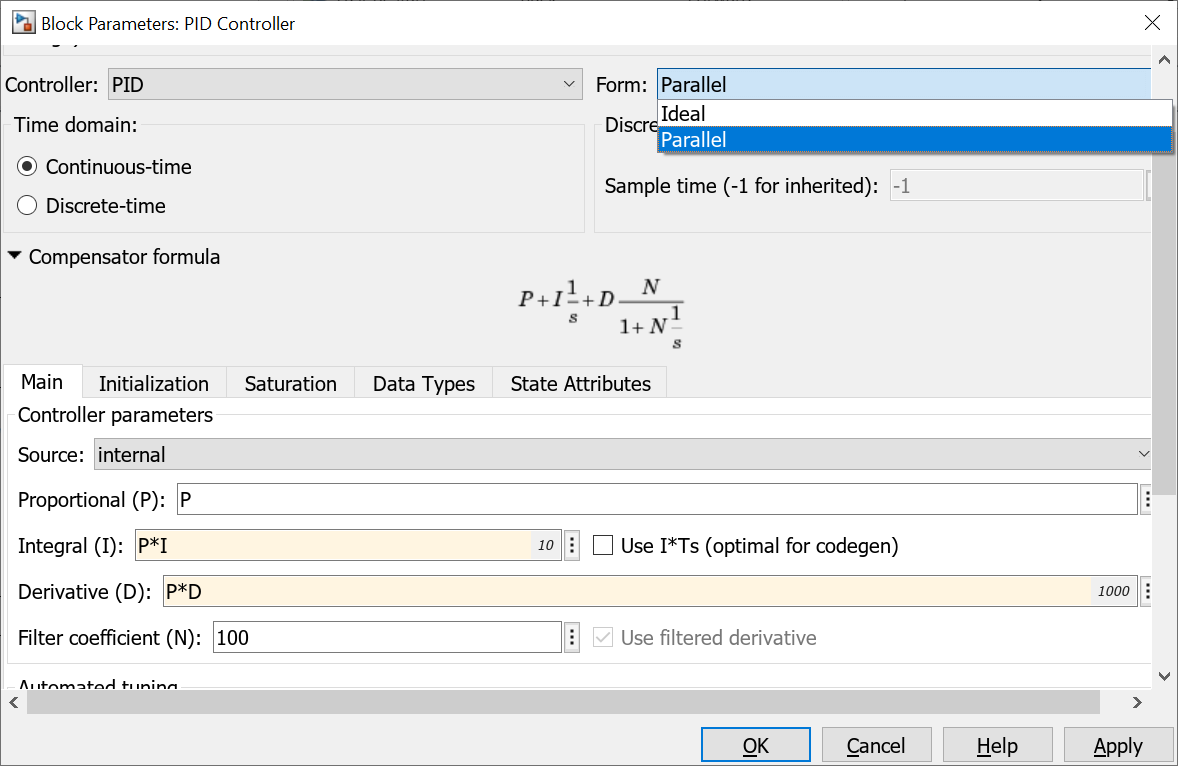
\includegraphics[width=\linewidth]{img/discussion_parallel_pid.png}
    \caption{Compensating for integral and derivative terms in parallel PID controller.}
    \label{fig:parallel pid controller block parameters}
\end{figure}

Thus to compensate for the parallel PID controller
as an ideal PID controller,
we multiply the integral and derivative terms each by the proportional term
as seen in Fig.~\ref{fig:parallel pid controller block parameters}.

\subsection{Use in cruise controls}

Varying the PID parameters of the controller creates very different results, and which parameters you decide on depends on the application that you desire to create.

For example, a cruise control, I would say that the best control would be a control with $P < 10$, $I < 1$, and $D = 0$. This would create very steady curves with very little overshoot or change in magnitude which would be ideal for cruise control.

\subsection{Use in critical response systems}

On the other hand, a system that needs quick responses may want to use a much higher derivative term such as $D=100$. Depending on whether the system should take a longer time to return to equilibrium, in the case that this is required, then the system should also increase its integral term.

The trade off in a critical response system is likely to be overshoot (as a result of attempting to respond as quick as possible) and thus the settling time.

\subsection{More considerations}

It would have been interesting to program the PID Controller in Verilog,
but I do not know about Verilog's capabilities with floating-point representations of real numbers.
This would make for an interesting alternative solution though.

Also, I began attempting to do a Bode plot for tasks 01--03,
but I could not finish that task
as Matlab does not have a built-in numerical Laplace transform function
and building one myself would be well outside of the scope of this experiment.

\newpage
\printbibliography

\newpage
\appendix
\section{Appendix}\label{app}

\subsection{Task 00 -- Initial parameters, Matlab script}\label{sap:initial params}
\inputminted{matlab}{src/lab09_task00_initial_dc_motor_motor_params.m}

\hr{}

\subsection{Task 01 -- Varying proportional terms, Matlab script}\label{sap:vary p}
\inputminted{matlab}{src/lab09_task01_vary_p.m}

\hr{}

\subsection{Task 02 -- Varying proportional, integral terms, Matlab script}\label{sap:vary pi}
\inputminted{matlab}{src/lab09_task02_vary_i.m}

\hr{}

\subsection{Task 03 -- Varying derivative terms, Matlab script}\label{sap:vary d}
\inputminted{matlab}{src/lab09_task03_vary_d.m}

\hr{}

\subsection{Task 07 -- Step response of faster than cruise control-PID controller}\label{sap:faster than cruise, step response}
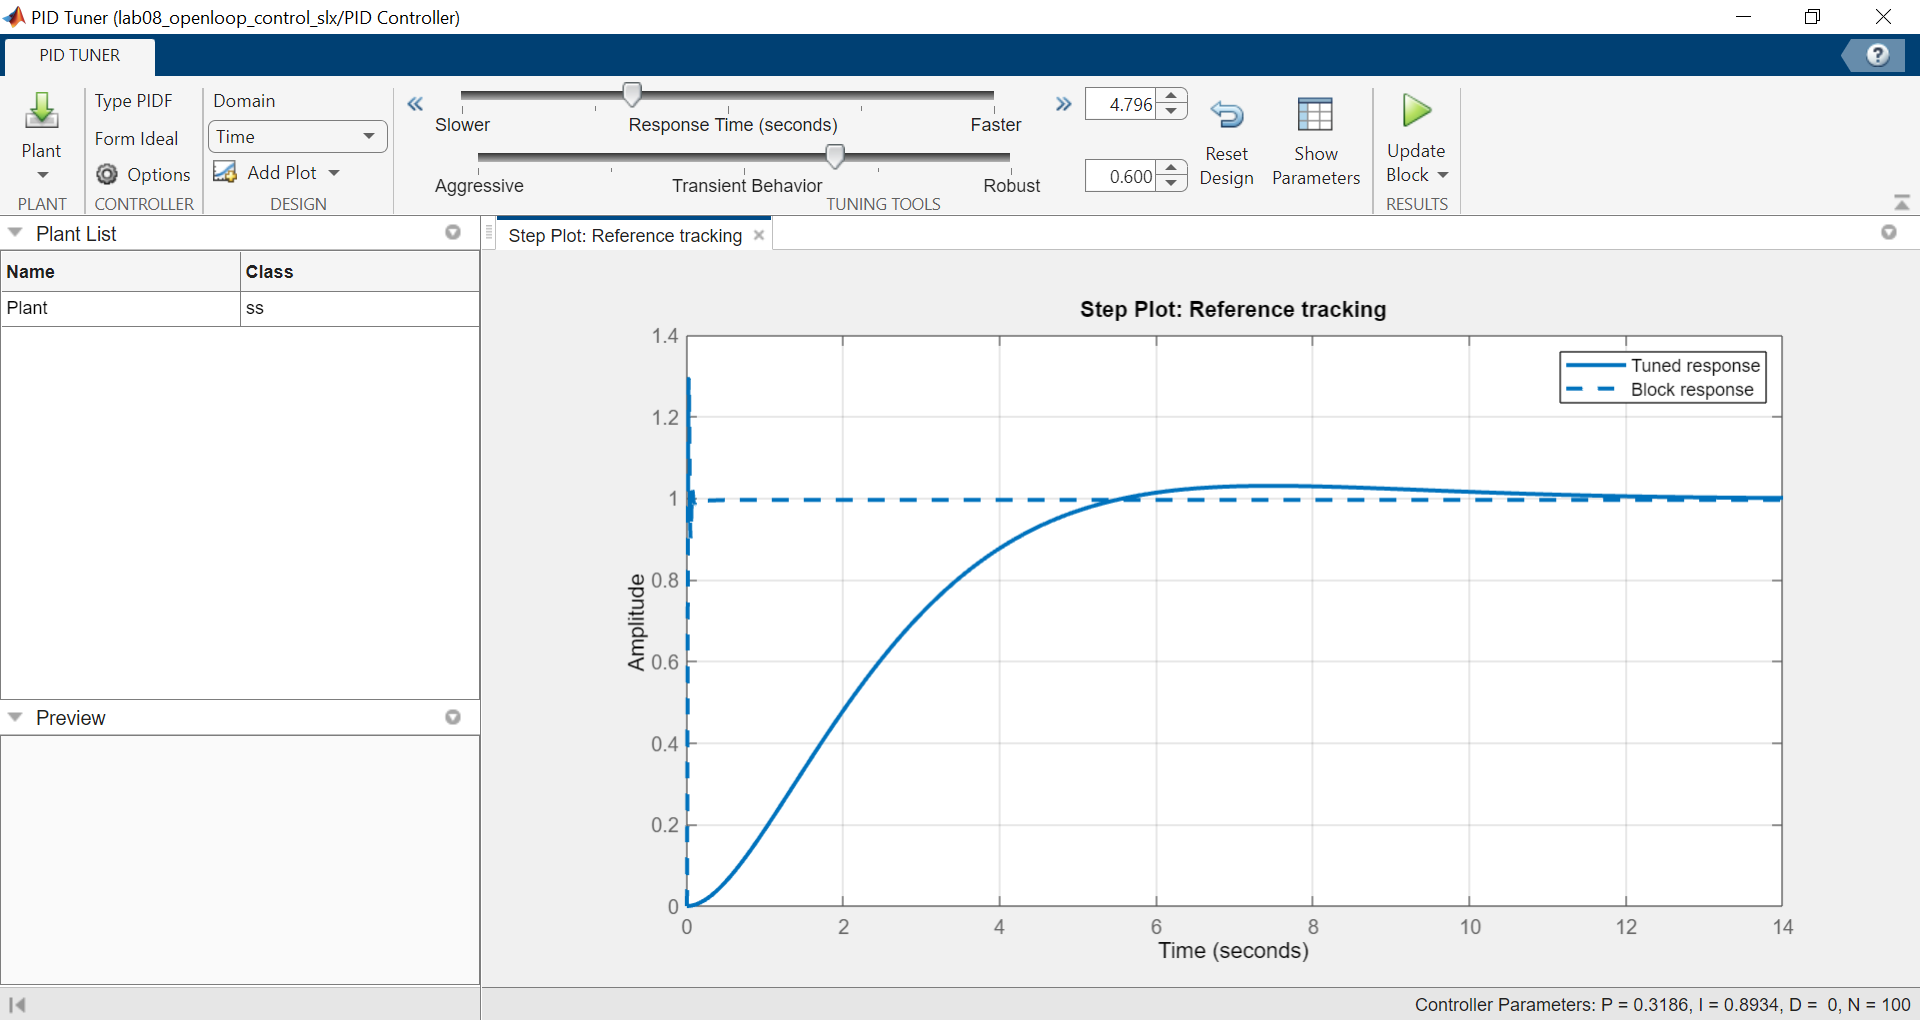
\includegraphics[width=\linewidth]{img/task07_025_cruise_control_faster.png}

\hr{}

\subsection{Task 07 -- Table of Parameters of cruise control-tuned PID controller, reference}\label{sap:tuned PID parameters reference table}
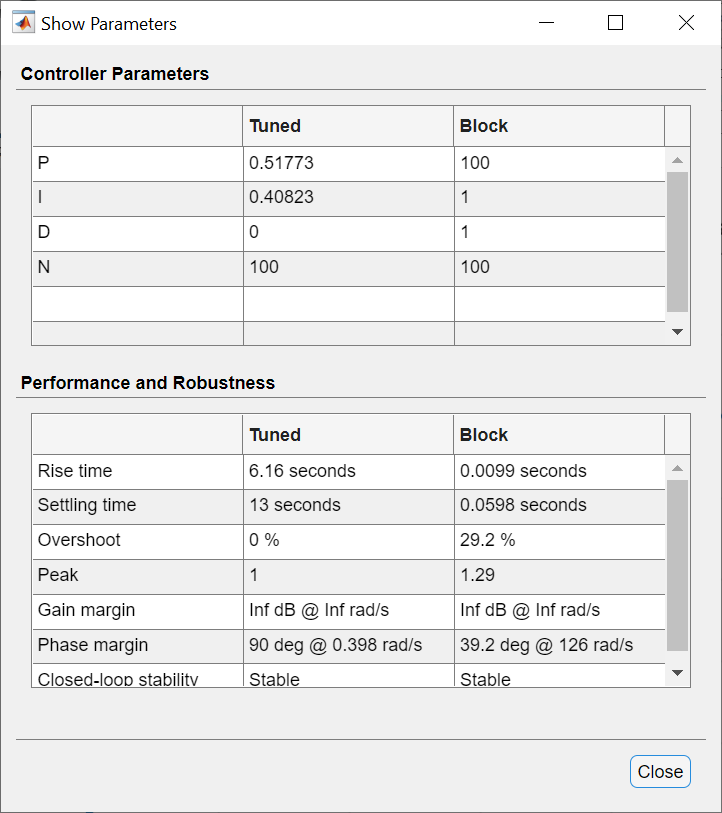
\includegraphics[width=\linewidth]{img/task07_030_cruise_control_table.png}

\hr{}

\subsection{Task 07 -- Table of Parameters of faster than cruise control-PID controller, reference}
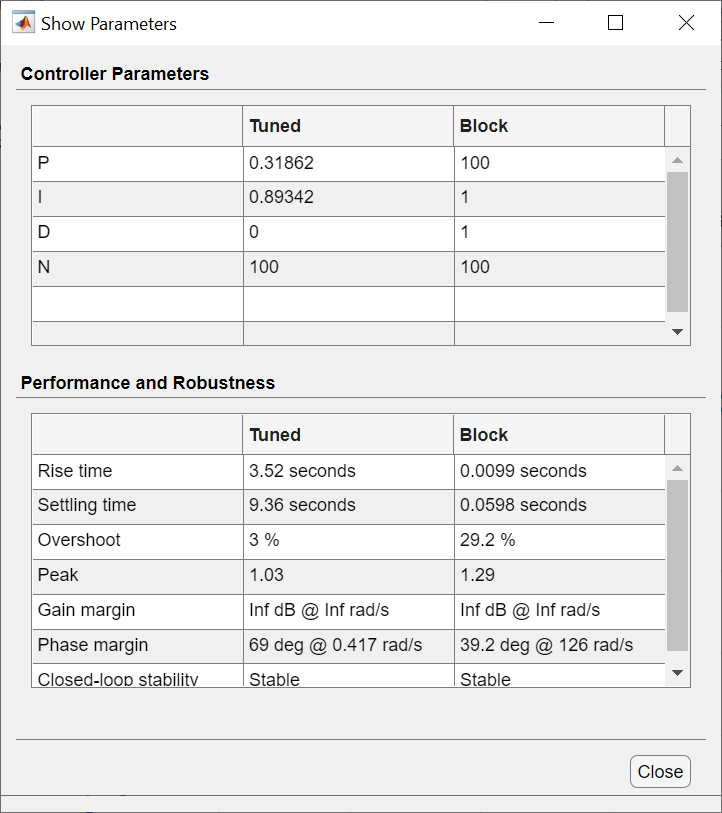
\includegraphics[width=\linewidth]{img/task07_035_cruise_control_faster_table.png}

\end{document}
